The next experiment we ran was to measure the amount of time it takes to run a procedure with 0-7 integer parameters. 
The measurement consists of resetting the timer, calling the function, and then having that function  read the instruction counter and return.
In addition, we measured the overhead for returning from a void function call by resetting the timer within the function and then reading the timer after returning.

On a procedure call, an ARM machine does the following actions:
\begin{itemize}
	\item Push registers to stack (Moving to L1 cache as a block, documented as 3 cycles)
	\item Copy first three passed arguments registers (1 cycles each since we pass constants)
	\item Copy additional arguments to memory (3 cycles per argument)
	\item Write new return pointer and stack pointer (2 cycles total)
\end{itemize}
Thus we suspect about 5 cycles for 0 argument functions and 1 cycle per argument up to 3 and then 3 cycles for subsequent arguments.
A return should be similar to a 1 argument function since it is poping off the stack (possibly a bit slower than pushing), copying the returned value, and then restoring the old return pointer and stack pointer.

\begin{figure}[h]
\centering
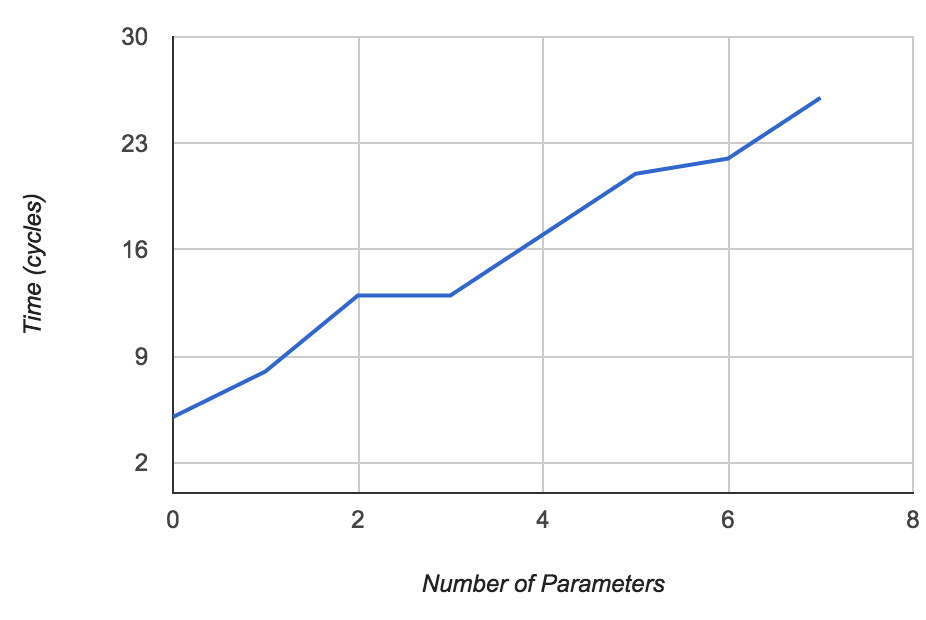
\includegraphics[scale=.5]{experiments/exp_1_2_fig.png}
\caption{Mean execution time vs number of parameters.    The standard deviation for all experiments was under 1 cycle}
\end{figure}

In the above figure we plot the mean procedure call time vs number of parameters.
From here we see that our prediction for zero arguments was exactly correct.  
Functions of 1-3 arguments was slower than we expected and plateaued between 2/3.
Functions of 4-7 arguments add about 3-4 cycles per argument inline with predictions.
The procedure return overhead is 13 cycles with standard deviation of 0 cycles, exactly inline with a function call of 2 arguments.
This is overhead over prediction is likely caused by additional slowness in popping vs pushing all the registers onto the stack.